%  !TEX root = ../main.tex
\section{Design of \alias}

\subsection{Overview}
\textbf{Design Goal.}
To manipulate ASRs while being used by users, adversaries shall create universal IAPs. However, they face the following challenges to obtain and deliver such perturbations:

% 这一段需要简化,特别是
\underline{\textit{Ultrasound Complexity (C1).}} Modeling the ultrasonic delivery is unprecedented compared to the audible-band RIR mimics, because ultrasound fundamentally differs from audible sound as listed in \textsection\ref{sec:ultrasound_observation}, including (i) ultrasound-induced anomalous noises, (ii) nonlinear distortion, (iii) varying sound field, and (iv) hardware-induced instability.

\blue{
\underline{\textit{User-ASR Connection (C2).}} ASR systems always respond to the user after receiving a command. Adversaries need to suppress the impact of \textit{user disruption}, i.e., break down the user-ASR connection by IAPs that can silence user's excessively long speech and remedy commands.}

\blue{
\underline{\textit{User Variation (C3).}} Since adversaries cannot exactly know the user speech's content, timing, or length, naively mixed speech signals will lead to undesirable ASR transcriptions. The tailored IAP needs to be universal while facing arbitrary user commands and superimposed time points.}

\underline{\textit{Physical Robustness (C4).}} The adversary also faces several factors that are variable in physical attacks, such as user loudness, hardware instability, and the user's environment (i.e., with different reverberations). We also extend the modulation method for reducing unexpected sound leakage.

\blue{To achieve adversaries' goal while addressing the aforementioned challenges, we propose \alias with unique technical design. This design includes: (1) tackling ultrasound complexity to deliver physically effective IAPs and therefore addressing \textit{user auditory} (cf.~\textsection\ref{sec:design_transformation}); (2) overcoming \textit{user disruption} to achieve real-time manipulation of ASR (cf.~\textsection\ref{sec:design_mute}, \ref{sec:design_universal}); (3) boosting attack stealthiness and practicality (cf.~\textsection\ref{sec:design_robust}). The optimization workflow of \alias is exhibited in Fig.~\ref{fig:design_overview}.}

\textbf{Problem Formalization.}
Unlike the audible-band AE attacks subject to stealthiness constraints, we achieve inaudible perturbations delivery using ultrasound modulation. Thus, we avoid the narrow constraints in Eq.~\ref{equ:audible_ae_formula}, e.g. $\epsilon<0.01$, where the IAP's optimization space can reach the maximum upper bound: $\delta\in[-1,1]^n$. We believe a broad optimization space possesses more feasible solutions, facilitating a universal attack. Combined with our core objective: fooling ASRs to recognize the superimposed speech of user voice and perturbation $x+\delta$ as the adversary-desired transcription $y_t$.
This basic idea can be optimized via the following formulation:
\begin{equation}
\begin{aligned}
    & {minimize}~ \mathcal{L}(f(x+\delta), y_t)\\
    & {s.t.}~ \delta \in [-1,1]^n ~{and}~ x+\delta \in [-1,1]^n
\end{aligned}
\label{equ:inaudible_formula}
\end{equation}

\subsection{Ultrasonic Transformation Modeling}\label{sec:design_transformation}
As shown in Fig.~\ref{fig:design_ufr}, our modeling exploits the \circled{5}additive property of the baseband audio $m$'s nonlinear transformation $H(f)m(f)$ and the ultrasound-induced anomalous noise $n$, and then \circled{6}yields estimated audio $\hat{m}=H(f)m(f)+n$ that is highly similar to the actual recorded audio $\widetilde{m}$.
In this subsection, we elaborate on our divide-and-conquer strategy of implementing ultrasonic transformation modeling that overcomes problems (i)-(iii) corresponding to \textit{ultrasound complexity (C1)}. Based on this, we can deliver physically effective IAPs via the steps \circled{1}$\sim$\circled{3} in Fig.~\ref{fig:design_overview}. We address the problem (iv) in \textsection\ref{sec:design_robust}. % We review the classical modeling failure and challenges of ultrasonic delivery in \textsection\ref{sec:preliminary}. The design should break down the barriers due to the ultrasound nature.

\subsubsection{Tackling Anomalous Noises}\label{sec:design_noise}
Ultrasound-based attacks modulate the baseband $m$ with $s(t)={A}{[1+m(t)]}c(t)$, where regardless of the energy of $m$, the carrier signal $c(t)=cos\omega_{c}t$ always emits and forces the microphone diaphragm into vibration, appearing abnormal noises~\cite{li2023learning}. 
Our experiment also demonstrates that although the recorded $s$ varies with $m$, the anomalous noise pattern is almost decided by the carrier. 
The nature of the ultrasound field further results in noise variation with different injection angles $\theta$ and distances $d$, showing irregular patterns. Therefore, due to such variation, neural networks fail to learn a stable mapping of the digital-to-physical domain.
We denote the noise $n(\theta,d)=f_n(\theta,d,s)$, where $f_n$ is the projection of the ultrasound signal $s$ to the recorded abnormal noise $n$ at different positions. 
In practice, an attacker can sample the variable anomalous noises by simply emitting the ultrasonic carrier. We collect a lightweight noise dataset using 25~kHz ultrasound (without modulation) of 1m at varying angles, forming a set $U_n$ of 25 pieces of 10-second noises.


\subsubsection{Ultrasonic Frequency Response}\label{sec:design_ufr}
Recalling the reasons for LTI system-based RIR's failure in \textsection\ref{sec:classic_rir} of modeling unprecedented ultrasonic delivery, except for anomalous noises, the inability to describe the nonlinear demodulation process is also a key factor. 
The adversaries aim to achieve robust and adaptive attacks with minimal effort, i.e., building an efficient transformation that can well estimate the demodulated pattern of a given digital perturbation after ultrasonic delivery in Fig.~\ref{fig:design_ufr} (red box). 
Fig.~\ref{fig:design_ufr} also depicts the recorded audio derived after inaudible signal injection, whose energy is clearly concentrated in the low-frequency band compared to the original audio~\cite{roy2018inaudible}.
Although nonlinearity exists, we are driven to obtain an ultrasonic frequency response (UFR) that characterizes the inaudible acoustic energy conversion at different frequencies.

\begin{figure}[t]
	\centering
	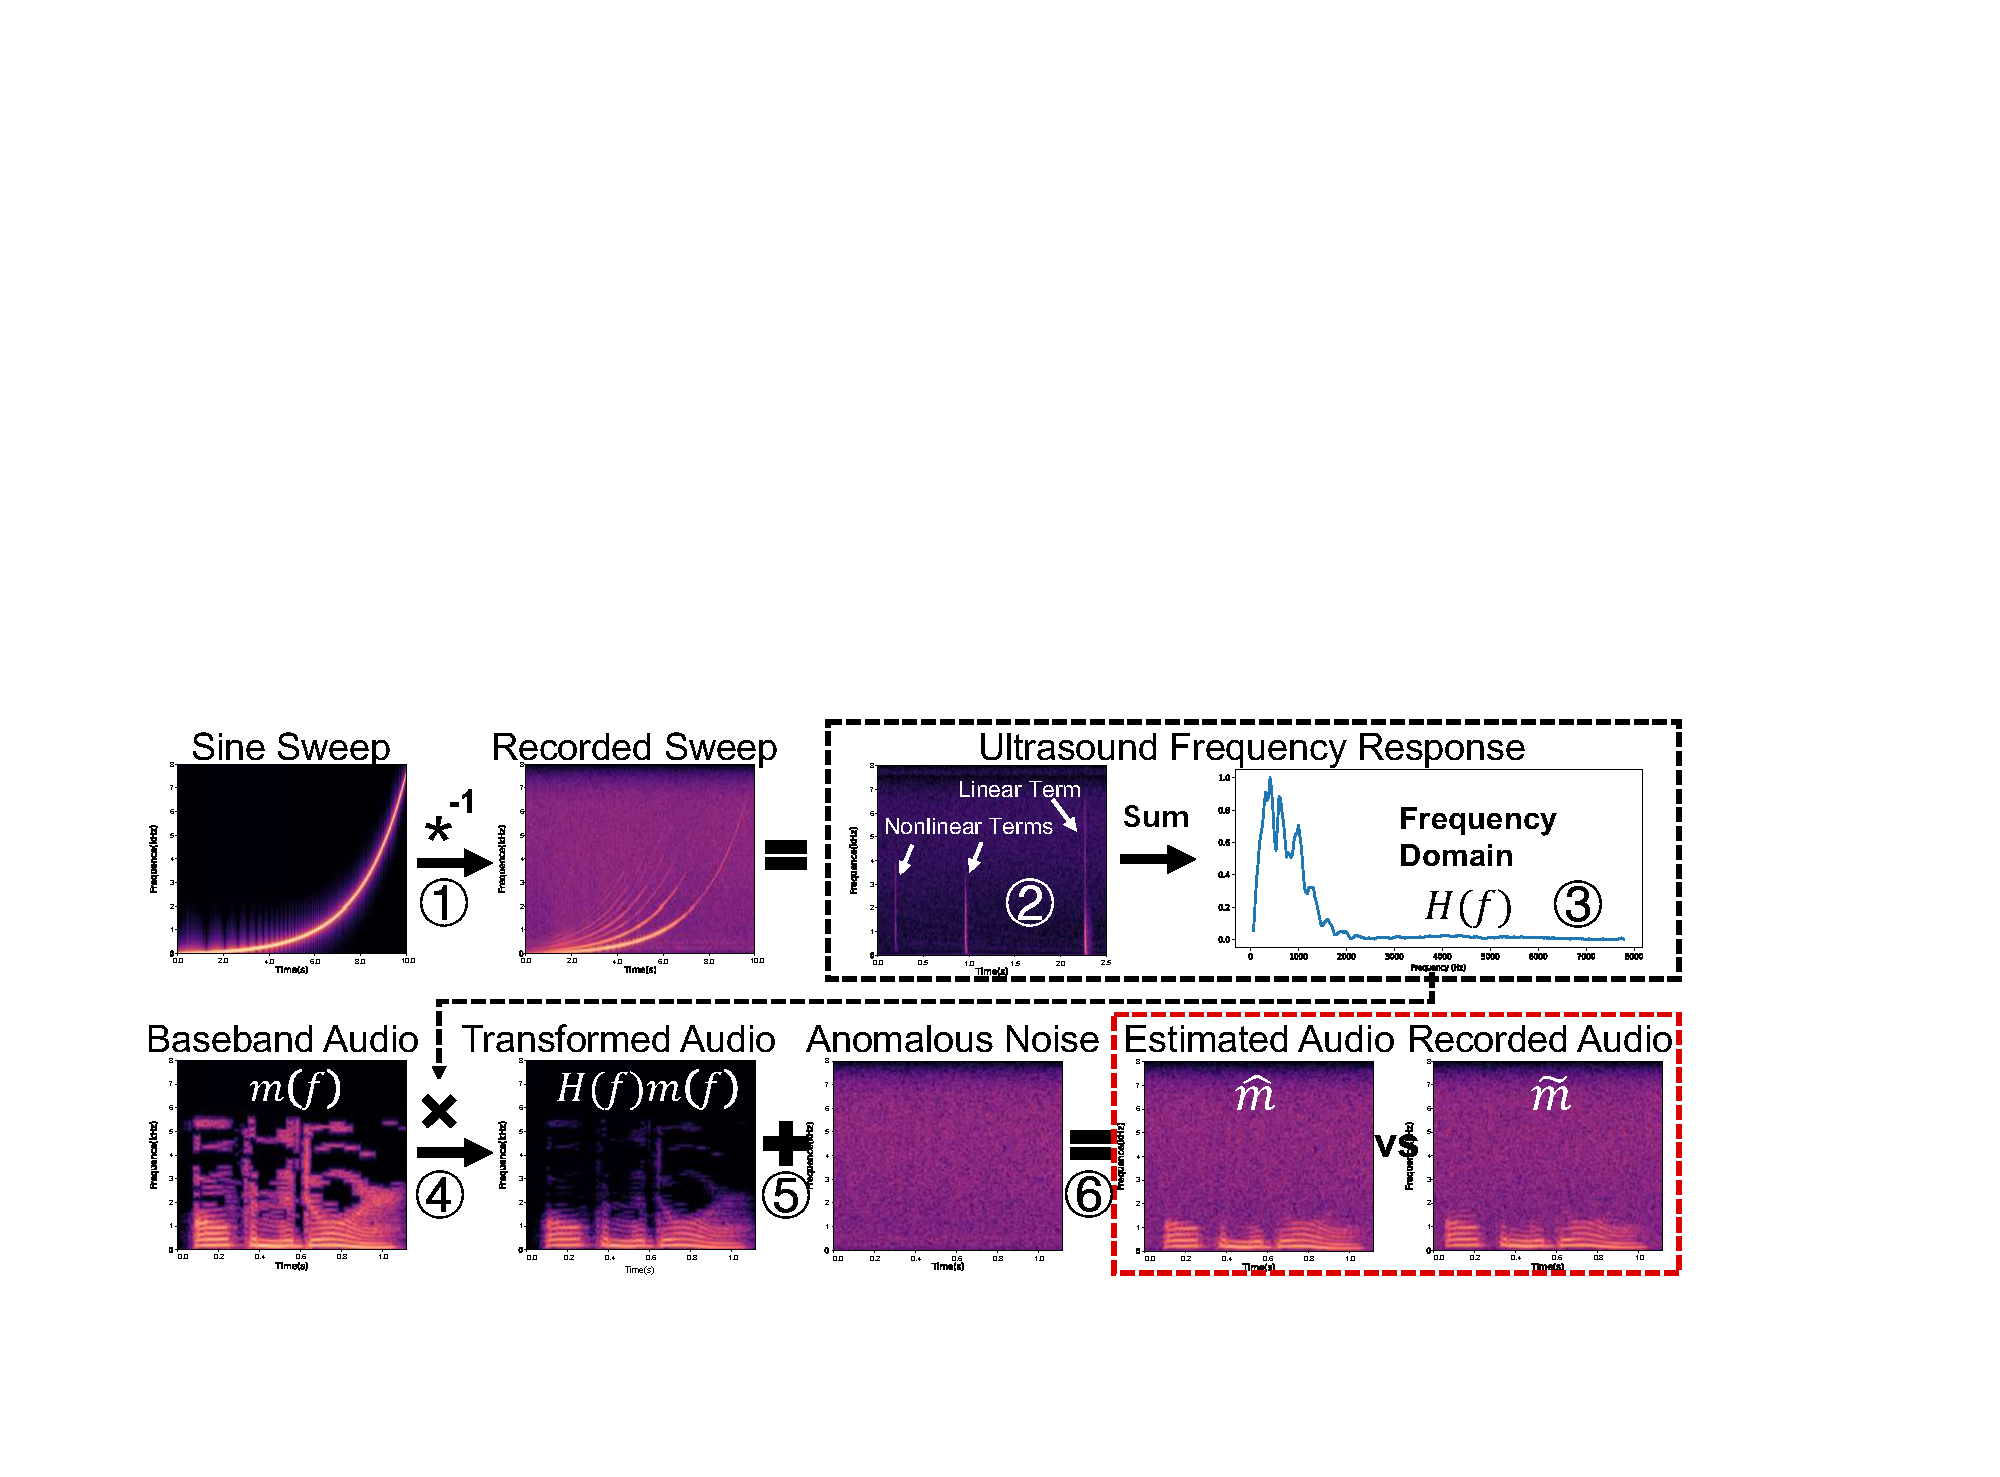
\includegraphics[width=0.48\textwidth]{design_ufr2.pdf}
	\caption{\label{fig:design_ufr}Ultrasonic transformation modeling. \textbf{1st row:} Procedure to obtain the ultrasonic frequency response (UFR). \textbf{2nd row:} High similarity between the estimated audio and actually recorded audio (the red box) proves its effectiveness.}
	\vspace{-15pt}
\end{figure}

We first overcome ultrasound-induced noises that hinder us from obtaining an accurate frequency response by adopting the sine sweep technique~\cite{farina2007advancements}, which can ignore components uncorrelated to the sweep signal during processing. We use it to generate a fast 10s sweep ranging from 50$\sim$7800~Hz, which is carefully chosen for diminishing hardware imperfection, and record it on the receivers, shown in Fig.~\ref{fig:design_ufr}\circled{1}. 
Thus, we can obtain the UFR $H(f)$ by deconvolution ($\ast^{-1}$). Notably, as shown in Fig.~\ref{fig:design_ufr}\circled{2}, it does shield the effects of noises and focuses on the frequency response measurement, which decouples the linear and nonlinear terms. We sum these terms up in Fig.~\ref{fig:design_ufr}\circled{3}, forming a holistic frequency-domain UFR of the received perturbations $\delta$ as $\overline{\Delta}(f)=H(f)\Delta(f)$, where $\Delta(f)=\mathcal{F}(\delta(t))$; $\mathcal{F}$ means Fourier Transform.


\subsubsection{Enabling Location-Variable} 
Uneven ultrasound field makes MLP-based method in \textsection\ref{sec:classic_nn} difficult to estimate transformation from arbitrary-position attack. As for efficient UFR, we believe that combining it with ultrasound $s(d,t)$ propagation process~\cite{holm2019waves} will empower to render more adaptive attacks:
\begin{equation}\label{equ:dis_filter}
    H(f,d) = H(f)\cdot e^{-a_0{\omega_c}^n d},~n\in[1,2]
\end{equation}
where $a_0$ is a medium-dependent attenuation parameter, $\omega_c$ is the carrier's frequency.
\blue{
Moreover, the energy variation caused by different injection angles is hard to model under such a changing sound field. We overcome this issue by conducting sine sweeps at different angles $\theta$ similar to \textsection\ref{sec:design_noise} and get 25 pieces of 10-second sweep clips.
Consequently, the collection of a complete set of UFRs and anomalous noises for subsequent optimization requires approximately 8.3 minutes.
Overall, with a pair of UFR $H_{\theta}(f,d)$ and noise clip $n(\theta,d)$ from the same location, we can well estimate the digital perturbation into its recording. However, to obtain a location-variable perturbation, we shall modify the expression of Eq.~\ref{equ:inaudible_formula} and find the perturbation via robust training:
}
\begin{equation}
    \underset{\delta}{argmin} \underset{h_{\theta} \sim U_H, n \sim U_n}{\mathbb{E}}\left[\mathcal{L}(f(x+h_{\theta}(d)\ast\delta+n), y_t\right]
\end{equation}
where we use time-domain expression $h_{\theta}(d)\ast\delta$ to indicate the transformed perturbation's waveform, as $H_{\theta}(f,d)\Delta(f)=\mathcal{F}[h_{\theta}(t,d)\ast\delta(t)]$ obeys the time convolution theorem.
We randomly select the UFR $H_{\theta}(f,d)$ and noise $n$ pairs from $U_H$ and $U_n$ during the optimization process to mimic actually delivering the inaudible adversarial perturbation at different locations. 
As we fully take ultrasound's inaudibility advantages, the experiment results also validate the optimization space is large enough to craft a robust perturbation effective under varying UFRs and noises.

 
\begin{figure*}[t]
	\centering
	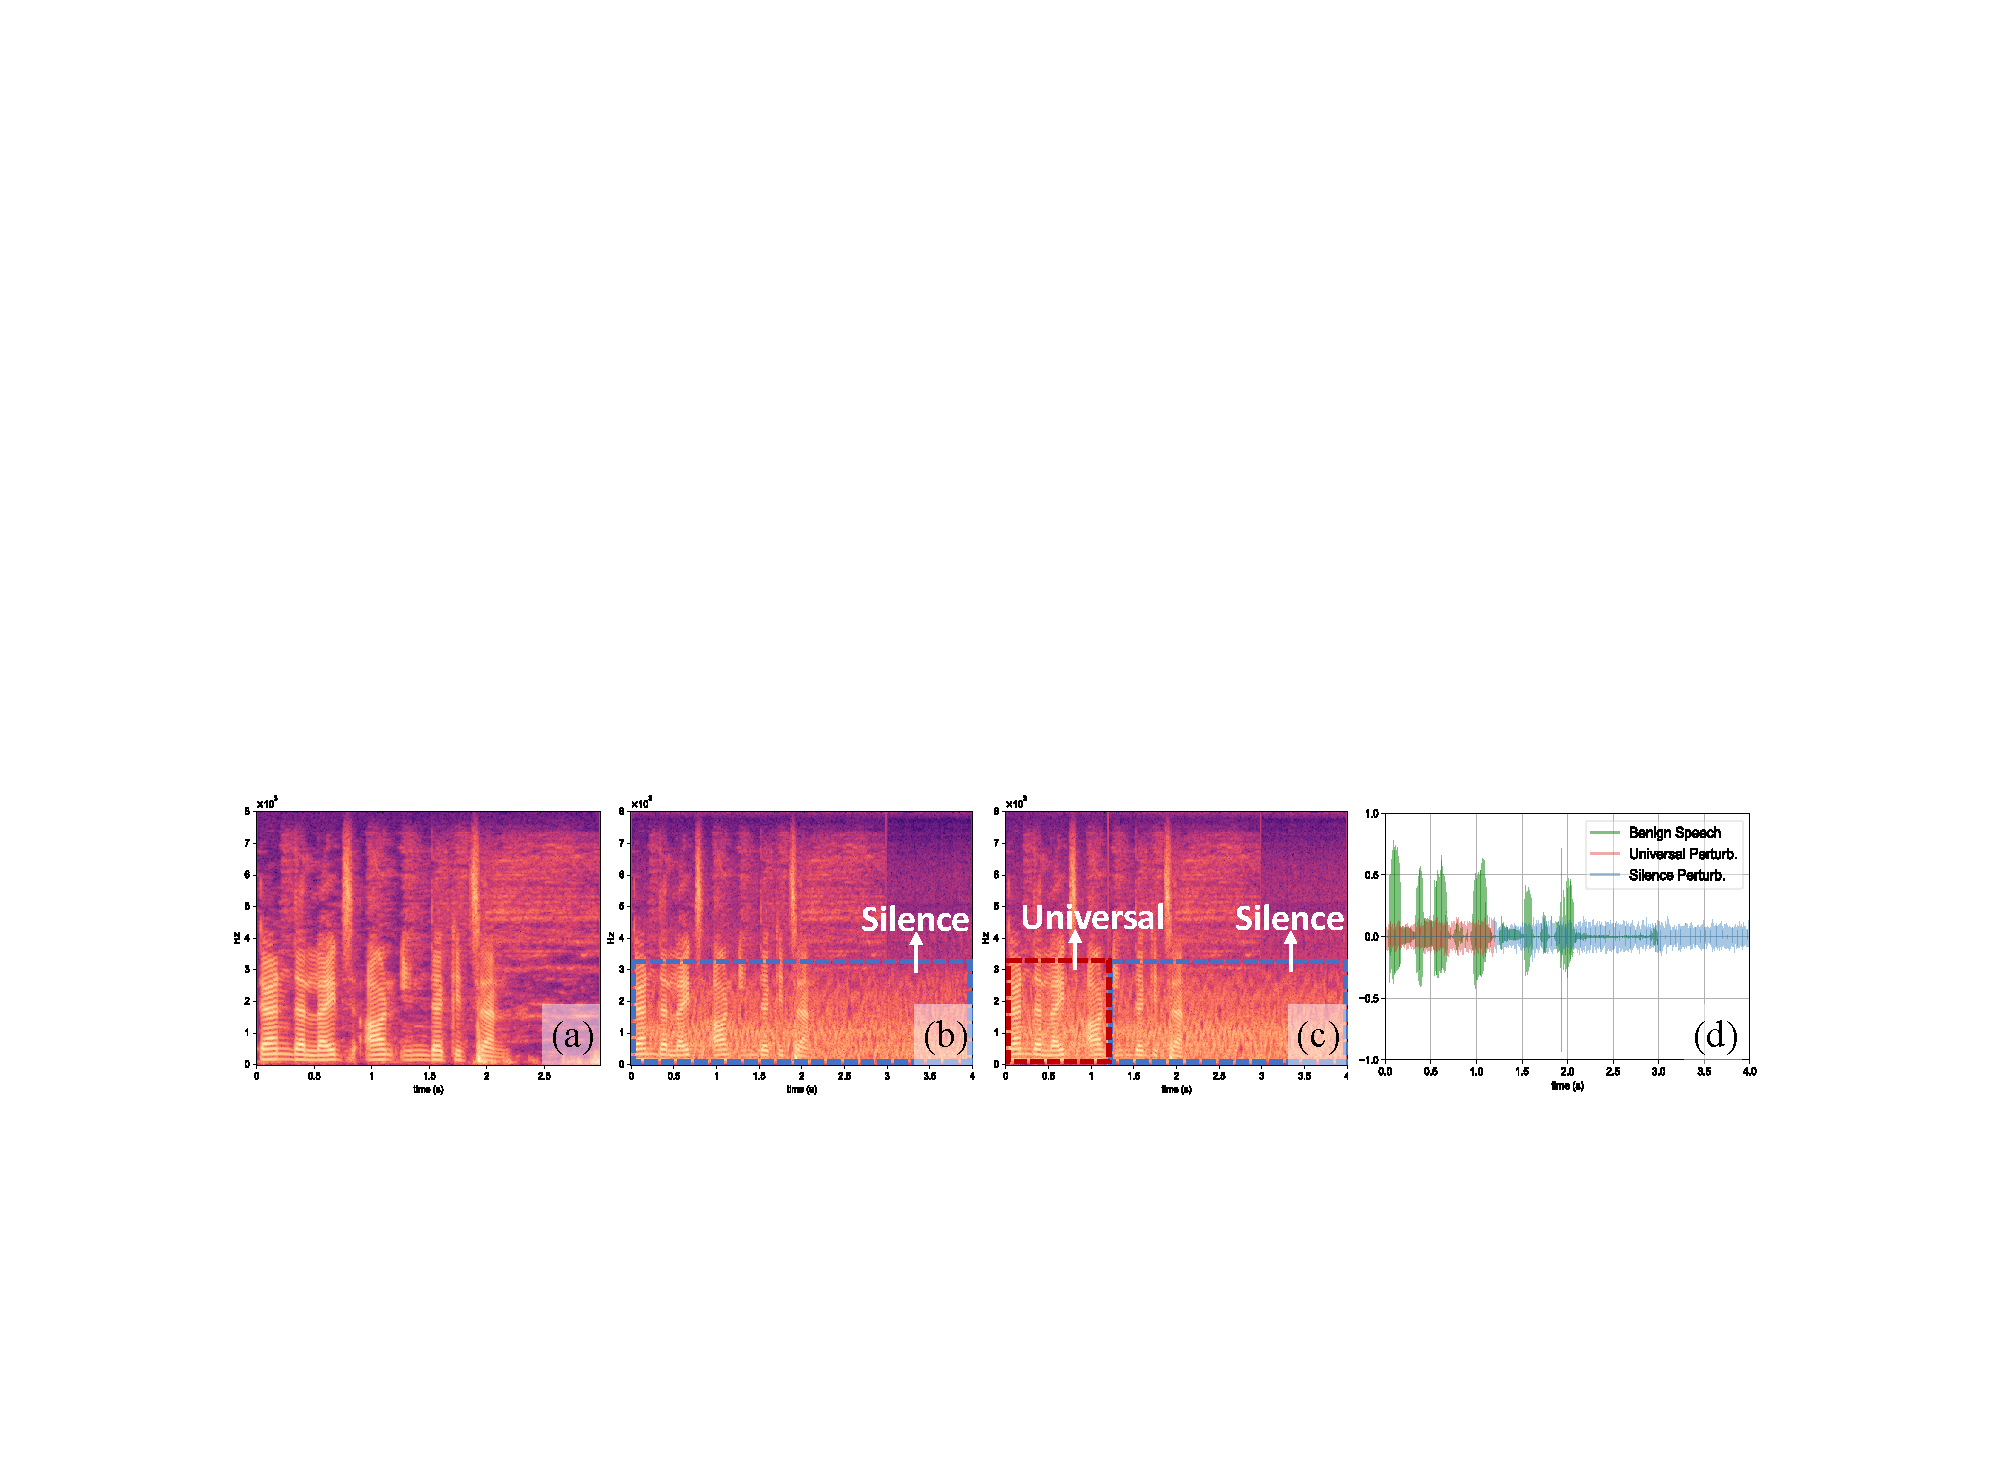
\includegraphics[width=0.8\textwidth]{perturbation_diagram.pdf}
        \vspace{-7pt}
	\caption{Diagram of \alias attacking a benign speech (a) with the silence (b) and universal goals in an \textit{alter-and-mute} manner (c\&d).}    %大图名称
	\label{fig:design_attack}    %图片引用标记
	\vspace{-15pt}
\end{figure*}

\subsection{\blue{Silence Perturbation}}\label{sec:design_mute}
\blue{Given the failures of prior works faced with \textit{user disruption}, specifically \ding{203} the challenge of excessively long instructions, and \ding{204} the potential counteraction through remedy commands, we believe that the solution lies in silencing the user instructions, i.e., breaking down the user-ASR connection when necessary.
Based on our ultrasonic transformation modeling, adversaries can materialize physically effective silence perturbations.
These perturbations can alter arbitrary user instructions to blank (`` '') in a targeted manner, effectively rendering the ASR system unresponsive to the user instructions.
We observe that implementing silence perturbations offers several advantages, including:
(1) When altering long user commands with short target intent, such as ``start recording'' (case \ding{203}). The silence perturbation can be linked alongside the universal perturbation in an \textit{alter-and-mute} fashion (cf. \textsection\ref{sec:design_universal}) so that the ASR will output adversary-desired transcription;
(2) it guarantees that users cannot meddle in running malicious operations by issuing remedy commands (case \ding{204}), even if they notice the presence of attacks; (3) it can render ASR services in the denial-of-service condition, preventing users from using them normally.}
Fig.~\ref{fig:design_attack}(b) depicts the diagram of a robust silence perturbation $\xi$, which is expected to superimpose over any benign content like Fig.~\ref{fig:design_attack}(a) and leads the final transcription of ASR to blank $y_b$ (`` '').  The length of $\xi$ is empirically set to 5s based on our experiments, for which we balance the duration of common speech instructions and the optimization overhead. For the case of excessively long user utterances, we address them in the generation process by repeating the perturbation.
\blue{To craft such a content-agnostic $\xi$, we improve the penalty-based expectation function to find the silence perturbation over a group of common voice commands $U_x$, as shown in Fig.~\ref{fig:design_overview}\circled{4}.}
\begin{equation}
    % \underset{\xi} {argmin}~\mathcal{L}\{f[\mathcal{S}_{x}+h_{\theta}(d)\ast\xi+n], y_b\}
    \underset{\xi}{argmin} \underset{h_{\theta} \sim U_H, n \sim U_n, x\sim U_x}{\mathbb{E}}[\mathcal{L}(f(\mathcal{S}_{x}+{h_{\theta}(d)\ast\xi+n}), y_b)]
\end{equation}
\blue{where $\mathcal{S}_{(\cdot)}$ means randomly shifting the user utterances $x$ for introducing randomness to the superimposed time within a preset $T$:100~ms. $U_x$ is elaborated in the experimental setup \textsection\ref{sec:eval_dataset}. It is more practical than the case where an AE and user speech are required to be perfectly aligned. The details of content-agnostic and synchronization are given in \textsection\ref{sec:design_universal}.}


\subsection{Universal Perturbation}\label{sec:design_universal}
\blue{Different from the proof of concept of universal AEs against a CNN-based speech command classification model presented in~\cite{li2020advpulse} by exploiting the temporal insensitivity of CNNs, the RNN-based models widely deployed on commercial ASR services are more difficult to attack.
This difficulty arises because end-to-end ASRs, such as DeepSpeech~\cite{amodei2016deep}, employ connectionist temporal classification (CTC) that calculates the loss between a continuous speech feature sequence and a target transcription, making it context-dependent. Consequently, when introducing subtle perturbations in different contexts, it is often difficult to ensure that the CTC losses of multiple mixed signals will simultaneously converge to the desired target.}

\subsubsection{\blue{Content-Agnostic}}
\blue{We believe that the reasons why previous audible-band AEs struggle to tamper with large amount of speech content are two-fold: \textit{user auditory} and \textit{user disruption}. 
To avoid being noticed by users, prior adversarial perturbations are limited by imperceptibility constraints and signal forms (e.g., with short length and subtle amplitude). Consequently, these perturbations are fragile and easily defensible. In contrast, our IAP delivery is completely inaudible via ultrasound modulation. Thus, the perturbation's length and amplitude are unconstrained, maximizing its optimization space. We fully use the advantages to generate a universal perturbation that can alter substantial short utterances into adversary-desired intent, e.g., a 1.2s $\delta$ tailored for “open the door”.}

\blue{
However, for excessively long speech or possible subsequent remedy commands in user-present scenarios (\textit{user disruption} \ding{203}-\ding{204}), the adversary should resort to the silence perturbation in \textsection\ref{sec:design_mute}, which can cooperate well with the universal perturbation in an \textit{alter-and-mute} manner.
As depicted in Fig.~\ref{fig:design_attack}(c) and (d), when the universal perturbation $\delta$ is combined with a well-trained silence perturbation $\hat{\xi}$, the former can apply to alter the user commands, and the latter will mute the subsequent user commands or remedies.}
As illustrated in Fig~\ref{fig:design_overview}\circled{4}, we determine the optimal $\delta$ by optimizing the following expectation function:
\begin{equation}
    \underset{\delta}{argmin} \underset{h_{\theta} \sim U_H, n \sim U_n, x\sim U_x}{\mathbb{E}}[\mathcal{L}(f(x+{h_{\theta}(d)\ast\overline{\delta:\hat{\xi}}+n}), y_t)]
    \vspace{-2pt}
\end{equation}
\blue{where {\scriptsize$\overline{\delta:\hat{\xi}}$} means the universal perturbation $\delta$ followed by a crafted silence perturbation $\hat{\xi}$. $U_x$ is the same subset used for generating silence perturbations, whose details are given in  \textsection\ref{sec:eval_dataset}.}

\subsubsection{Synchronization-Aided}\label{sec:sync_free}
Although the universal perturbation can deceive the ASR with any victim’s speech into adversary-desired intent, an adversary can hardly deliver attacks synchronously when the victim vocalizes. 
\blue{Out of attack practicality, we propose a VAD-based synchronization mechanism to achieve real-time manipulation, which avoids continuous AE broadcasting or assuming an adversary always ready for attacking.
Specifically, we employ a microphone to record the user's voice. Once detecting the user's speech via voice activity detection (VAD), our program automatically triggers the emission of the prepared perturbation. 
Based on our experiments, the delay is impacted by three stages of our real-time pipeline: (1) from user vocalizing to being detected by the running VAD program (5$\sim$20~ms); (2) software-to-hardware IAP triggering (5$\sim$15~ms); (3) ultrasound propagation (0$\sim$30~ms). Due to the delay uncertainty, we consider bringing the time randomness of a range $T$ into our optimization, whose upper bound is empirically set to 100~ms. For a direct reference, the average overall delay when attacking at 4m is around 27~ms, far below the maximum tolerable delay (100~ms) preset during optimization.
Particularly, the recording of user speech can also be utilized to present a more covert attack by inaudibly replaying user-desired commands, as ``\textit{Man-in-the-middle Attack}'' stated in \textsection\ref{sec:threat_model}.
By integrating the above-mentioned optimization objectives, we further craft the universal IAP through the below expectation:}
\begin{equation}\label{equ:sync_attack}
    \underset{\delta}{argmin} \underset{h_{\theta} \sim U_H, n \sim U_n, x\sim U_x}{\mathbb{E}}[\mathcal{L}(f(x+\mathcal{S}_{h_{\theta}(d)\ast\overline{\delta:\hat{\xi}}+n}), y_t)]
\end{equation}
where $\mathcal{S}_{(\cdot)}$ mimics \alias can be superimposed on victim speech at random time points (Fig.~\ref{fig:design_overview}\circled{4}) within the preset $T$.


\subsection{Physical Robustness}\label{sec:design_robust} % 幅值鲁棒的优点是否是已经优化过的?
\subsubsection{Loudness Adaptive and Hardware Instability} When conducting physical attacks, \alias is able to handle the challenges of ultrasound nature based on our digital-to-physical transformation in \textsection\ref{sec:design_transformation}. However, the loudness of the victim's speech varies with context or emotion, and hardware instability still exists.
These will result in difficulty maintaining our inaudible perturbation in effectively altering the victim's voice if the mutual energy relationship between the two is inconsistent with the optimization process.
As shown in Fig.~\ref{fig:design_overview}\circled{5}, we introduce relative volume augmentation into the crafting process, which exploits a hyper-parameter $\beta$ denoting a range of user speech's volume and thereby brings randomness to the mutual relationship between user voice and perturbation.

\subsubsection{Attack at Different Environments} Although ultrasound-based attacks directly inject into recording devices' microphones and are reverberation-free, the audible-band human voice still goes through multi-path reflections and ambient noises in different environments. To alter user commands regardless of the impact of scenes, we apply random RIR and noise clips from the Aachen Impulse Response (AIR) Database~\cite{jeub2009binaural} in Fig.~\ref{fig:design_overview}\circled{6}, including small, medium, large rooms and corridors for user speech augmentation.

\subsubsection{\blue{Single-Sideband Extension}}\label{sec:SSB}
\blue{
Although \alias can achieve real-time manipulation of the ASR output very covertly using sophisticated devices (e.g., narrowband ultrasonic transducers and signal generators) at long distances through windows or doors, we aim to accomplish highly stealthy attacks even in close proximity to the victim by utilizing everyday-life loudspeakers or portable attack devices.
However, the simple amplifiers, sound cards, and off-the-shelf loudspeakers exhibit poor suppression of intermodulation and harmonics of high-frequency DSB-AM signals. Namely, they present increased nonlinearity, resulting in sound leakage (cf. \textsection\ref{sec:discuss}). 
To enable attacks with portable devices and loudspeakers (cf. \textsection\ref{sec:portable_attack}), we adopt single-sideband amplitude modulation (SSB-AM), which removes one of the sidebands based on the Hilbert transform~\cite{ziemer2006principles}. 
Compared to DSB-AM, SSB-AM has only half the bandwidth, rendering higher transmission efficiency. 
Importantly, it mitigates the intermodulation between different sideband frequencies, making the sound less prone to leakage than DSB-AM at the same energy level. Specifically, we employ upper sideband modulation (USB-AM), formalized as $S(t)=m{cos\omega_{c}t}-\hat{m}{sin\omega_{c}t}+cos\omega_{c}t$, rather than lower sideband modulation (LSB-AM), as the former exhibits better inaudibility in our experiments and more details are given in Appendix  \textsection\ref{append:SSB}.}

Overall, the algorithm of \alias is described in Algorithm \ref{algo1}, Appendix \textsection\ref{append:algo1}, where we demonstrate the optimization process of crafting \alias from scratch.


